\documentclass[a4paper,11pt]{article}
\input{/home/tof/Documents/Cozy/latex-include/preambule_doc.tex}
\input{/home/tof/Documents/Cozy/latex-include/preambule_commun.tex}
\newcommand{\showprof}{show them}  % comment this line if you don't want to see todo environment
\setlength{\fboxrule}{0.8pt}
\fancyhead[L]{\fbox{\Large{\textbf{Tris 02}}}}
\fancyhead[C]{\textbf{Exercices tris}}
\newdate{madate}{10}{09}{2020}
%\fancyhead[R]{\displaydate{madate}} %\today
%\fancyhead[R]{Seconde - SNT}
\fancyhead[R]{Première - NSI}
%\fancyhead[R]{Terminale - NSI}
\fancyfoot[L]{\vspace{1mm}Christophe Viroulaud}
\AtEndDocument{\label{lastpage}}
\fancyfoot[C]{\textbf{Page \thepage/\pageref{lastpage}}}
\fancyfoot[R]{\includegraphics[width=2cm,align=t]{/home/tof/Documents/Cozy/latex-include/cc.png}}
\usepackage{tikz}

\begin{document}
\begin{exo}
En considérant que la durée d'exécution du tri par sélection est proportionnelle à $n^2$ et qu'il prend 6,8 secondes pour trier 16000 éléments, combien de temps prendra-t-il pour trier 1 million d'éléments?
\end{exo}
\begin{exo}
    On considère le tableau:
    \begin{center}
    \begin{lstlisting}[language=Python]
    [3, 4, 1, 7, 2]
    \end{lstlisting}
    \end{center}
\begin{enumerate}
    \item Détailler les étapes du tri par sélection sur ce tableau.
    \item Détailler les étapes du tri par insertion sur ce tableau.
\end{enumerate}
\end{exo}
\begin{exo}
Pour comparer si deux tableaux de même longueur sont identiques, c’est-à-dire s'ils contiennent les mêmes éléments, une stratégie consiste à d'abord les trier puis comparer chaque élément un à un.
\begin{enumerate}
    \item Construire la fonction \textbf{\texttt{comparer(tab1: list, tab2: list) $\rightarrow$ bool}} qui compare les éléments des tableaux un à un et renvoie \textbf{\texttt{True}} s'ils sont identiques.
    \item Utiliser la fonction tri par insertion pour trier les tableaux:
    \begin{itemize}
        \item \textbf{\texttt{[3, 5, 9, 0, 1, 8, 2]}},
        \item \textbf{\texttt{[9, 5, 3, 2, 8, 1, 0]}}.
    \end{itemize}
    \item Comparer les deux tableaux avec la fonction \textbf{\texttt{comparer}}.
\end{enumerate}
\end{exo}
\begin{exo}
Le tri par insertion vu en cours, effectue un tri en place. Pour garder inchangées les données initiales, il faut construire un nouveau tableau.
\begin{enumerate}
    \item Écrire la fonction \textbf{\texttt{tri\_insertion(tab: list) $\rightarrow$ list}} qui crée un nouveau tableau trié à partir des éléments de \emph{tab}. La fonction parcourra \emph{tab}, copiera l'élément de rang \emph{i} à la fin du nouveau tableau puis positionnera cet élément à sa bonne position.
    \item Construire par compréhension un tableau de dix éléments aléatoires compris entre 0 et 100.
    \item Tester la fonction de tri sur ce tableau.
\end{enumerate}
\end{exo}
\begin{exo}
\begin{enumerate}
    \item Adapter le tri par insertion vu en cours pour trier le tableau de tuples suivants en fonction du premier élément des tuples:
    \begin{center}
    \begin{lstlisting}[language=Python]
tab = [(5, "a"), (8, "b"), (1, "e"), (5, "d"), (7, "f"), (8, "c")]
    \end{lstlisting}
    \end{center}
    \item Un \emph{tri stable} conserve l'ordre initial des éléments de même valeur. Le tri par insertion est-il stable?
\end{enumerate}
\end{exo}
\begin{exo}
\begin{enumerate}
    \item Construire par compréhension un tableau de cent éléments aléatoires compris entre 0 et 10.
    \item En s'aidant du tri par insertion, écrire la fonction \textbf{\texttt{max\_occurrences(tab: list) $\rightarrow$ int}} qui renvoie l'élément le plus présent dans le tableau. \underline{Indication:} dans un tableau trié les éléments identiques se suivent. 
\end{enumerate}
\end{exo}
\begin{exo}
Le tri à bulles \emph{fait remonter} les plus grands éléments d'un tableau, comme des bulles d'air qui remonteraient à la surface d'un liquide. Le code \ref{bulle} présente la première itération qui permet de propager le plus grand élément en dernière place du tableau. Il suffit ensuite d'effectuer une deuxième itération pour propager le deuxième plus grand élément en avant-dernière position.
    \begin{center}
        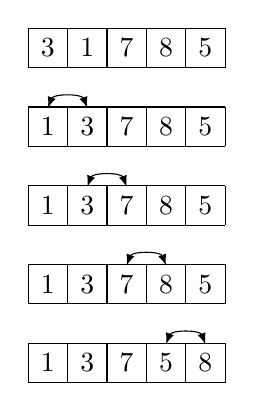
\begin{tikzpicture}[scale=0.5]
            \draw (0,0) grid (5,1);
            \node at(0.5,0.5) {3};
            \node at(1.5,0.5) {1};
            \node at(2.5,0.5) {7};
            \node at(3.5,0.5) {8};
            \node at(4.5,0.5) {5};

            
            \draw (0,-2) grid (5,-1);
            \node (1) at(0.5,-1.5) {1};
            \node (2)at(1.5,-1.5) {3};
            \node at(2.5,-1.5) {7};
            \node at(3.5,-1.5) {8};
            \node at(4.5,-1.5) {5};
            \draw[<->,>=latex] (1.north)to[bend left=70](2.north);

            \draw (0,-4) grid (5,-3);
            \node at(0.5,-3.5) {1};
            \node (3)at(1.5,-3.5) {3};
            \node (4)at(2.5,-3.5) {7};
            \node at(3.5,-3.5) {8};
            \node at(4.5,-3.5) {5};
            \draw[<->,>=latex] (3.north)to[bend left=70](4.north);

            \draw (0,-6) grid (5,-5);
            \node at(0.5,-5.5) {1};
            \node at(1.5,-5.5) {3};
            \node (5)at(2.5,-5.5) {7};
            \node (6)at(3.5,-5.5) {8};
            \node at(4.5,-5.5) {5};
            \draw[<->,>=latex] (5.north)to[bend left=70](6.north);
    
            \draw (0,-8) grid (5,-7);
            \node at(0.5,-7.5) {1};
            \node at(1.5,-7.5) {3};
            \node at(2.5,-7.5) {7};
            \node (7)at(3.5,-7.5) {5};
            \node (8)at(4.5,-7.5) {8};
            \draw[<->,>=latex] (7.north)to[bend left=70](8.north);
        \end{tikzpicture}
        \captionof{code}{Tri à bulles - première itération de la boucle externe}
        \label{bulle}
        \end{center}

\begin{enumerate}
    \item Écrire la fonction \textbf{\texttt{echanger(tab: list, i: int, j: int) $\rightarrow$ None}} qui permute les éléments d'indices \emph{i} et \emph{j} de \emph{tab}.
    \item Écrire la fonction \textbf{\texttt{tri\_bulles(tab: list) $\rightarrow$ None}} qui implémente le tri à bulles. Cette fonction utilisera la fonction \textbf{\texttt{echanger}}.
    \item Construire par compréhension un tableau de vingt éléments d'entiers aléatoires compris entre 0 et 1000.
    \item Tester la fonction de tri sur ce tableau.
\end{enumerate}
\end{exo}
\end{document}